\documentclass[../main.tex]{subfiles}
%% \graphicspath{{\subfix{../images/}}}

\begin{document}

To finalize our insight of how PNC works, we need to describe the build process from high-level perspective:
\begin{enumerate}
    \item \textbf{Trigger a build}\\
    Build is triggered (almost exclusively) either from PNC UI or Bacon CLI. In both cases, this results in Orch's \textit{trigger build} endpoint being called. Every build is configured by its build configuration containing all the necessary information, e.g.:
    \begin{itemize}
        \item \textbf{upstream repository:} publicly available repository with source code, e.g. \url{https://github.com/wildfly/wildfly}
        \item \textbf{git reference:} (branch, tag or commit) revision which will be used to clone source code, e.g. \textit{34.0.0.Final}
        \item \textbf{build type:} either Maven, Gradle, NPM or SBT
        \item \textbf{build environment:} build environment used in build container
        \item \textbf{build script:} script executed in build container, e.g. \textit{mvn clean deploy}
    \end{itemize}

    \item \textbf{Clone repository from upstream}\\
    Repour clones specified upstream repository locally into the container environment in which it runs. Subsequently, it calls the corresponding manipulator based on the build type (for instance, for Maven build type, PME manipulator is picked).

    \item \textbf{Alignment process}\\
    Manipulator configured from repour communicates with DA to perform both version increment and depdencies alignment.

    \item \textbf{Push alignment changes}\\
    Once manipulator successfully finishes, alignment changes are pushed into downstream repository.

    \item \textbf{Create build container}\\
    Create the environment for the build itself based on build environment from build configuration.

    \item \textbf{Clone alignment changes}\\
    Before build container runs the build itself, it needs to clone alignment changes from downstream repository pushed by repour in step 4.

    \item \textbf{Run a build}\\
    Run build script from build configuration. During the build, build container communicates with artifact repository in order to fetch artifacts.

    \item \textbf{Store built artifacts}\\
    Once a build succeeds, its produced artifacts need to be stored in artifact repository in order to be accessible by subsequent builds.

    \item \textbf{Save build result into DB}\\
    Save all the build-related data into the orch database. This involves information like used build configuration, artifacts produced by the build, or artifacts used by the build.
    
\end{enumerate}

The whole build process is also visualized by BPMN diagram\footnote{\url{https://miro.com/diagramming/what-is-bpmn/}} shown in Figure \ref{fig:build-process-bpmn}.

\begin{figure}
  \begin{center}
    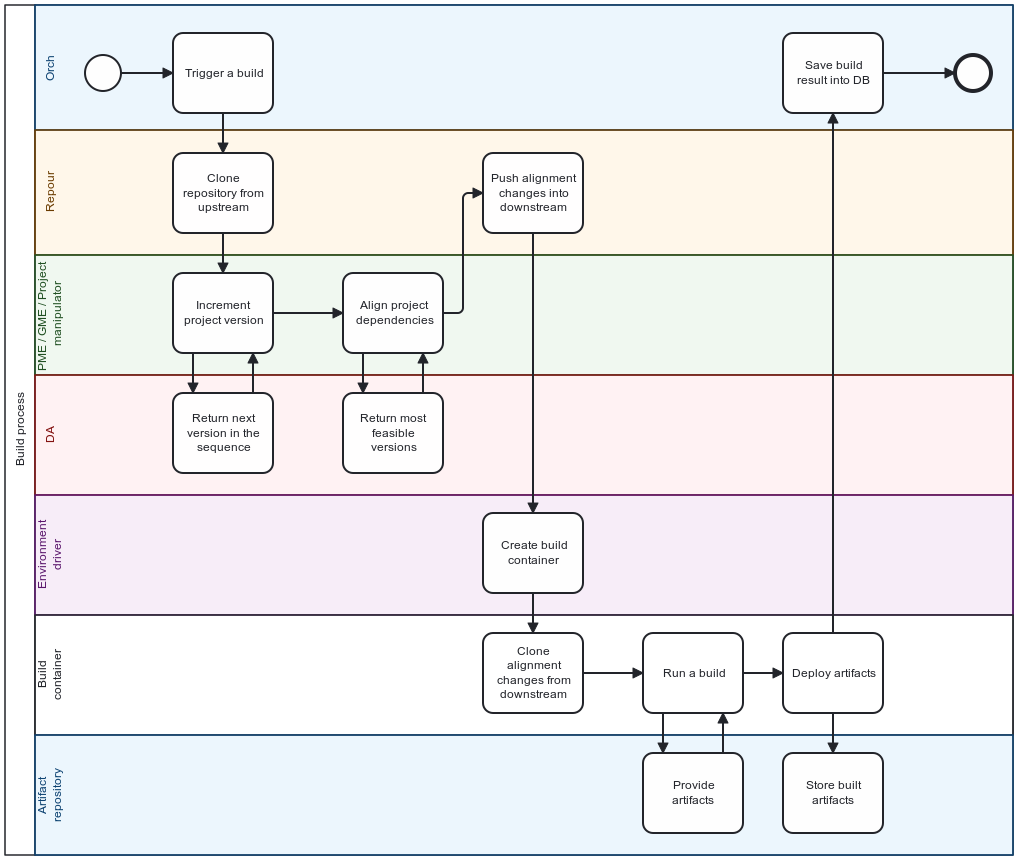
\includegraphics[width=\textwidth]{images/build-process-bpmn.png}
  \end{center}
  \caption{BPMN build process diagram}
  \label{fig:build-process-bpmn}
\end{figure}

\end{document}
